\documentclass[10pt,a4paper,titlepage]{article}

\usepackage[english]{babel}
\usepackage[T1]{fontenc}
\usepackage[utf8x]{inputenc}
\usepackage[a4paper,includeheadfoot,dvipdfm,pdftex]{geometry}
\usepackage{pslatex}
\usepackage{booktabs}
\usepackage{longtable}
\usepackage{multicol}
\usepackage{tabularx}
\usepackage{fancyhdr}
\usepackage{ifthen}
\usepackage[table]{xcolor}
\usepackage{hyphenat}
\usepackage{tikz}
\usepackage{pgfplots}
\usepackage{hyperref}
\hypersetup{
    breaklinks = true,
    colorlinks = true,
    urlcolor   = blue,
    citecolor  = black,
    filecolor  = black,
    linkcolor  = black
}
\geometry{
    top      = 20mm,
    left     = 20mm,
    right    = 20mm,
    bottom   = 50mm,
    headsep  = 10mm,
    footskip = 10mm
}
\setlength{\parindent}{0cm}

\pagestyle{fancy}
\fancyhfoffset[R]{0mm}

\voffset-10mm
\topmargin0mm
\headsep10mm
\headheight20mm
\hbadness=10000
\vbadness=10000

\usepackage{caption}
\captionsetup{
   labelfont = bf,
   textfont  = it,
}

\newif\ifcopyright
\copyrightfalse % \copyrighttrue for copyright, \copyrightfalse for no copyright

\newif\ifwatermark
\watermarkfalse % \watermarktrue for watermark, \watermarkfalse for no watermark

\newif\iflogaxis
\logaxistrue % \logaxistrue for logarithmic scale, \logaxisfalse for "normal" scale

\iflogaxis
    \def\loglabel{ [log]}
\else
    \def\loglabel{}
\fi

\fancyhf{}
\renewcommand{\headrulewidth}{0pt}

\ifcopyright
    \newcommand{\mycopyright}{%
        {\small Copyright \copyright\ __COPYRIGHT__}%
    }
    % Copyright on the title page
    \fancypagestyle{empty}{\cfoot{\mycopyright}}
\fi

\cfoot{%
    {\bf\thepage}\\%
    \ifcopyright
        \mycopyright
    \fi
}

\ifwatermark
    \usepackage{draftwatermark}
    \SetWatermarkText{__WATERMARK__}
    \SetWatermarkLightness{.9}
\fi

\newcommand{\HRule}[1]{\rule{\linewidth}{#1}}

\newcolumntype{M}{>{\raggedleft\arraybackslash}m{.3\textwidth}}
\newcolumntype{R}{>{\raggedleft\arraybackslash}X}
\newcolumntype{L}{>{\raggedright\arraybackslash}X}

% New page for each section
\let\stdsection\section
\renewcommand\section{\clearpage\stdsection}

% Alternate row color
\newcommand\altrowcolorodd{__TABLE_ODD_COLOR__}
\newcommand\altrowcoloreven{__TABLE_EVEN_COLOR__}

% Fill in color for charts
\newcommand\chartcolor{__CHART_COLOR__}

% pgfplots configuration
\pgfset{
    bar width = 14pt,
}

\pgfplotsset{
    compat = newest,
    width = \textwidth,
    height = .3\textheight,
    x tick label style = {/pgf/number format/1000 sep=},
    legend style = {
        at = { (0.5, -0.15) },
        anchor = north,
        legend columns = -1
    },
    ybar,
    xtick = data,
    point meta = rawy,
    axis on top,
    axis x line* = bottom,
    axis y line* = left,
    y axis line style = {opacity=0},
    yticklabels = {\empty},
    ytick style = {draw=none},
    enlarge y limits = {upper, value=.11},
    nodes near coords,
    nodes near coords align = {vertical},
}

\iflogaxis
\pgfplotsset{ymin = 1}
\else
\pgfplotsset{ymin = 0}
\fi

% longtable
\let\oldlongtable\longtable
\let\endoldlongtable\endlongtable
\renewenvironment{longtable}{%
    \rowcolors{2}{\altrowcoloreven}{\altrowcolorodd}%
    \oldlongtable%
}{%
    \endoldlongtable%
    \global\rownum=0\relax%
}
% tabular
\let\oldtabular\tabular
\let\endoldtabular\endtabular
\renewenvironment{tabular}{%
    \rowcolors{2}{\altrowcoloreven}{\altrowcolorodd}%
    \oldtabular%
}{%
    \endoldtabular%
    \global\rownum=0\relax%
}
% tabularx
\let\oldtabularx\tabularx
\let\endoldtabularx\endtabularx
\renewenvironment{tabularx}{%
    \rowcolors{2}{\altrowcoloreven}{\altrowcolorodd}%
    \oldtabularx%
}{%
    \endoldtabularx%
    \global\rownum=0\relax%
}

\title{%
    \HRule{0.5pt}\\[0.2cm]
    \Huge\textbf{__TITLE__}\\[0.2cm]
    %__BEGIN_FILE_REQUIRED__
    \Large\texttt{__FILENAME__}\\
    %__END_FILE_REQUIRED__
    %__BEGIN_DB_REQUIRED__
    \Large __DBTYPE__ Database\\
    \texttt{__FILENAME__}\\[0.2cm]
    \large __PERIOD__
    %__END_DB_REQUIRED__
    \HRule{2pt}\\[3.0cm]
    %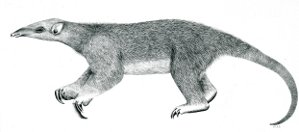
\includegraphics[scale=1.4]{img/anteater.jpg}\\
}
\author{__AUTHOR__}

\begin{document}

%\tracingall

\pagenumbering{alph}

\maketitle

\tableofcontents

\pagenumbering{arabic}

\section{Summary}
    \begin{itemize}
        %__BEGIN_FILE_REQUIRED__
        \item Filename: {\tt __FULLNAME__}
        \item MD5: {\tt __MD5SUM__}
        \item File size: __FILESIZE__
        %__END_FILE_REQUIRED__
        %__BEGIN_DB_REQUIRED__
        \item __DBTYPE__ Database: {\tt __FULLNAME__}
        %__END_DB_REQUIRED__
        \item Number of packets: __NUMPKTS__
        \item Number of bytes: __NUMBYTES__
        \item First packet seen: __FIRSTPKT__
        \item Last packet seen: __LASTPKT__
        \item Capture duration: __SECONDS__ seconds __DURSTR__
        \item Number of distinct IP addresses: __DISTIP__
            \begin{itemize}
                \item __PRIVIP__ private
                \item __PUBIP__ public
                \item __DISTIP4__ IPv4
                \item __DISTIP6__ IPv6
            \end{itemize}
        %\item Min/Max/Average flow duration:
        %\item Min/Max/Average packets per flow:
        %\item Min/Max/Average bytes per flow:
    \end{itemize}

\section{Top __TABLE_N__ IP Addresses}

        % Flows

        \begin{minipage}{.45\textwidth}
            \begin{tabular}{MMM}
                \toprule
                {\bf SrcIP} & {\bf Country} & {\bf Flows}\\
                \midrule
                %__SRCIP_CN_FLOWS__
                \bottomrule
            \end{tabular}
        \end{minipage}
        \hfill
        \begin{minipage}{.45\textwidth}
            \begin{tabular}{MMM}
                \toprule
                {\bf DstIP} & {\bf Country} & {\bf Flows}\\
                \midrule
                %__DSTIP_CN_FLOWS__
                \bottomrule
            \end{tabular}
        \end{minipage}

        \vspace{\belowdisplayskip}

        % Packets

        \begin{minipage}{.45\textwidth}
            \begin{tabular}{MMM}
                \toprule
                {\bf SrcIP} & {\bf Country} & {\bf Packets}\\
                \midrule
                %__SRCIP_CN_PKTS__
                \bottomrule
            \end{tabular}
        \end{minipage}
        \hfill
        \begin{minipage}{.45\textwidth}
            \begin{tabular}{MMM}
                \toprule
                {\bf DstIP} & {\bf Country} & {\bf Packets}\\
                \midrule
                %__DSTIP_CN_PKTS__
                \bottomrule
            \end{tabular}
        \end{minipage}

        \vspace{\belowdisplayskip}

        % Bytes

        \begin{minipage}{.45\textwidth}
            \begin{tabular}{MMM}
                \toprule
                {\bf SrcIP} & {\bf Country} & {\bf Bytes}\\
                \midrule
                %__SRCIP_CN_BYTES__
                \bottomrule
            \end{tabular}
        \end{minipage}
        \hfill
        \begin{minipage}{.45\textwidth}
            \begin{tabular}{MMM}
                \toprule
                {\bf DstIP} & {\bf Country} & {\bf Bytes}\\
                \midrule
                %__DSTIP_CN_BYTES__
                \bottomrule
            \end{tabular}
        \end{minipage}

%__BEGIN_COUNTRIES__
\section{Top __TABLE_N__ Countries}

        % Flows

        \begin{minipage}{.33\textwidth}
            \begin{tabularx}{.9\textwidth}{lR}
                \toprule
                {\bf Src Country} & {\bf Flows}\\
                \midrule
                %__SRC_CC_FLOWS__
                \bottomrule
            \end{tabularx}
        \end{minipage}
        \hfill
        \begin{minipage}{.33\textwidth}
            \begin{tabularx}{.9\textwidth}{lR}
                \toprule
                {\bf Src Country} & {\bf Packets}\\
                \midrule
                %__SRC_CC_PKTS__
                \bottomrule
            \end{tabularx}
        \end{minipage}
        \hfill
        \begin{minipage}{.33\textwidth}
            \begin{tabularx}{.9\textwidth}{lR}
                \toprule
                {\bf Src Country} & {\bf Bytes}\\
                \midrule
                %__SRC_CC_BYTES__
                \bottomrule
            \end{tabularx}
        \end{minipage}

        \vspace{\belowdisplayskip}

        % Destination Coutries

        \begin{minipage}{.33\textwidth}
            \begin{tabularx}{.9\textwidth}{lR}
                \toprule
                {\bf Dst Country} & {\bf Flows}\\
                \midrule
                %__DST_CC_FLOWS__
                \bottomrule
            \end{tabularx}
        \end{minipage}
        \hfill
        \begin{minipage}{.33\textwidth}
            \begin{tabularx}{.9\textwidth}{lR}
                \toprule
                {\bf Dst Country} & {\bf Packets}\\
                \midrule
                %__DST_CC_PKTS__
                \bottomrule
            \end{tabularx}
        \end{minipage}
        \hfill
        \begin{minipage}{.33\textwidth}
            \begin{tabularx}{.9\textwidth}{lR}
                \toprule
                {\bf Dst Country} & {\bf Bytes}\\
                \midrule
                %__DST_CC_BYTES__
                \bottomrule
            \end{tabularx}
        \end{minipage}
%__END_COUNTRIES__

\section{Top __CHART_N__ Ports}

    \subsection{Top __CHART_N__ TCP Ports}

        % Flows

        \begin{minipage}{.48\textwidth}
            \begin{tikzpicture}
                \iflogaxis
                    \begin{semilogyaxis}[
                \else
                    \begin{axis}[
                \fi
                    ylabel = {\bf Flows\loglabel},
                    xlabel = {\bf Destination Port},
                    symbolic x coords = {
                        %__TCP_DPORT_FLOWS__
                    };
                \iflogaxis
                    \end{semilogyaxis}
                \else
                    \end{axis}
                \fi
            \end{tikzpicture}
        \end{minipage}
        \hfill
        \begin{minipage}{.48\textwidth}
            \begin{tikzpicture}
                \raggedleft
                \iflogaxis
                    \begin{semilogyaxis}[
                \else
                    \begin{axis}[
                \fi
                    ylabel = {\bf Flows\loglabel},
                    xlabel = {\bf Source Port},
                    symbolic x coords = {
                        %__TCP_SPORT_FLOWS__
                    };
                \iflogaxis
                    \end{semilogyaxis}
                \else
                    \end{axis}
                \fi
            \end{tikzpicture}
        \end{minipage}

        % Packets

        \begin{minipage}{.48\textwidth}
            \begin{tikzpicture}
                \iflogaxis
                    \begin{semilogyaxis}[
                \else
                    \begin{axis}[
                \fi
                    ylabel = {\bf Packets\loglabel},
                    xlabel = {\bf Destination Port},
                    symbolic x coords = {
                        %__TCP_DPORT_PKTS__
                    };
                \iflogaxis
                    \end{semilogyaxis}
                \else
                    \end{axis}
                \fi
            \end{tikzpicture}
        \end{minipage}
        \hfill
        \begin{minipage}{.48\textwidth}
            \begin{tikzpicture}
                \iflogaxis
                    \begin{semilogyaxis}[
                \else
                    \begin{axis}[
                \fi
                    ylabel = {\bf Packets\loglabel},
                    xlabel = {\bf Source Port},
                    symbolic x coords = {
                        %__TCP_SPORT_PKTS__
                    };
                \iflogaxis
                    \end{semilogyaxis}
                \else
                    \end{axis}
                \fi
            \end{tikzpicture}
        \end{minipage}

        % Bytes

        \begin{minipage}{.48\textwidth}
            \begin{tikzpicture}
                \iflogaxis
                    \begin{semilogyaxis}[
                \else
                    \begin{axis}[
                \fi
                    ylabel = {\bf Bytes\loglabel},
                    xlabel = {\bf Destination Port},
                    symbolic x coords = {
                        %__TCP_DPORT_BYTES__
                    };
                \iflogaxis
                    \end{semilogyaxis}
                \else
                    \end{axis}
                \fi
            \end{tikzpicture}
        \end{minipage}
        \hfill
        \begin{minipage}{.48\textwidth}
            \begin{tikzpicture}
                \iflogaxis
                    \begin{semilogyaxis}[
                \else
                    \begin{axis}[
                \fi
                    ylabel = {\bf Bytes\loglabel},
                    xlabel = {\bf Source Port},
                    symbolic x coords = {
                        %__TCP_SPORT_BYTES__
                    };
                \iflogaxis
                    \end{semilogyaxis}
                \else
                    \end{axis}
                \fi
            \end{tikzpicture}
        \end{minipage}

    \subsection{Top __CHART_N__ UDP Ports}

        % Flows

        \begin{minipage}{.48\textwidth}
            \begin{tikzpicture}
                \iflogaxis
                    \begin{semilogyaxis}[
                \else
                    \begin{axis}[
                \fi
                    ylabel = {\bf Flows\loglabel},
                    xlabel = {\bf Destination Port},
                    symbolic x coords = {
                        %__UDP_DPORT_FLOWS__
                    };
                \iflogaxis
                    \end{semilogyaxis}
                \else
                    \end{axis}
                \fi
            \end{tikzpicture}
        \end{minipage}
        \hfill
        \begin{minipage}{.48\textwidth}
            \begin{tikzpicture}
                \raggedleft
                \iflogaxis
                    \begin{semilogyaxis}[
                \else
                    \begin{axis}[
                \fi
                    ylabel = {\bf Flows\loglabel},
                    xlabel = {\bf Source Port},
                    symbolic x coords = {
                        %__UDP_SPORT_FLOWS__
                    };
                \iflogaxis
                    \end{semilogyaxis}
                \else
                    \end{axis}
                \fi
            \end{tikzpicture}
        \end{minipage}

        % Packets

        \begin{minipage}{.48\textwidth}
            \begin{tikzpicture}
                \iflogaxis
                    \begin{semilogyaxis}[
                \else
                    \begin{axis}[
                \fi
                    ylabel = {\bf Packets\loglabel},
                    xlabel = {\bf Destination Port},
                    symbolic x coords = {
                        %__UDP_DPORT_PKTS__
                    };
                \iflogaxis
                    \end{semilogyaxis}
                \else
                    \end{axis}
                \fi
            \end{tikzpicture}
        \end{minipage}
        \hfill
        \begin{minipage}{.48\textwidth}
            \begin{tikzpicture}
                \iflogaxis
                    \begin{semilogyaxis}[
                \else
                    \begin{axis}[
                \fi
                    ylabel = {\bf Packets\loglabel},
                    xlabel = {\bf Source Port},
                    symbolic x coords = {
                        %__UDP_SPORT_PKTS__
                    };
                \iflogaxis
                    \end{semilogyaxis}
                \else
                    \end{axis}
                \fi
            \end{tikzpicture}
        \end{minipage}

        % Bytes

        \begin{minipage}{.48\textwidth}
            \begin{tikzpicture}
                \iflogaxis
                    \begin{semilogyaxis}[
                \else
                    \begin{axis}[
                \fi
                    ylabel = {\bf Bytes\loglabel},
                    xlabel = {\bf Destination Port},
                    symbolic x coords = {
                        %__UDP_DPORT_BYTES__
                    };
                \iflogaxis
                    \end{semilogyaxis}
                \else
                    \end{axis}
                \fi
            \end{tikzpicture}
        \end{minipage}
        \hfill
        \begin{minipage}{.48\textwidth}
            \begin{tikzpicture}
                \iflogaxis
                    \begin{semilogyaxis}[
                \else
                    \begin{axis}[
                \fi
                    ylabel = {\bf Bytes\loglabel},
                    xlabel = {\bf Source Port},
                    symbolic x coords = {
                        %__UDP_SPORT_BYTES__
                    };
                \iflogaxis
                    \end{semilogyaxis}
                \else
                    \end{axis}
                \fi
            \end{tikzpicture}
        \end{minipage}

\section{Top Protocols and Applications}

    % Flows

    \begin{minipage}{.48\textwidth}
        \begin{tikzpicture}
            \iflogaxis
                \begin{semilogyaxis}[
            \else
                \begin{axis}[
            \fi
                ylabel = {\bf Flows\loglabel},
                xlabel = {\bf Protocol},
                symbolic x coords = {
                    %__PROTO_FLOWS__
                };
            \iflogaxis
                \end{semilogyaxis}
            \else
                \end{axis}
            \fi
        \end{tikzpicture}
    \end{minipage}
    \hfill
    \begin{minipage}{.48\textwidth}
        \begin{center}
            \begin{tabularx}{.8\textwidth}{lR}
                \toprule
                {\bf Application} & {\bf Flows}\\
                \midrule
                %__APP_FLOWS__
                \bottomrule
            \end{tabularx}
        \end{center}
    \end{minipage}

    % Packets

    \begin{minipage}{.48\textwidth}
        \begin{tikzpicture}
            \iflogaxis
                \begin{semilogyaxis}[
            \else
                \begin{axis}[
            \fi
                ylabel = {\bf Packets\loglabel},
                xlabel = {\bf Protocol},
                symbolic x coords = {
                    %__PROTO_PKTS__
                };
            \iflogaxis
                \end{semilogyaxis}
            \else
                \end{axis}
            \fi
        \end{tikzpicture}
    \end{minipage}
    \hfill
    \begin{minipage}{.48\textwidth}
        \begin{center}
            \begin{tabularx}{.8\textwidth}{lR}
                \toprule
                {\bf Application} & {\bf Packets}\\
                \midrule
                %__APP_PKTS__
                \bottomrule
            \end{tabularx}
        \end{center}
    \end{minipage}

    % Bytes

    \begin{minipage}{.48\textwidth}
        \begin{tikzpicture}
            \iflogaxis
                \begin{semilogyaxis}[
            \else
                \begin{axis}[
            \fi
                ylabel = {\bf Bytes\loglabel},
                xlabel = {\bf Protocol},
                symbolic x coords = {
                    %__PROTO_BYTES__
                };
            \iflogaxis
                \end{semilogyaxis}
            \else
                \end{axis}
            \fi
        \end{tikzpicture}
    \end{minipage}
    \hfill
    \begin{minipage}{.48\textwidth}
        \begin{center}
            \begin{tabularx}{.8\textwidth}{lR}
                \toprule
                {\bf Application} & {\bf Bytes}\\
                \midrule
                %__APP_BYTES__
                \bottomrule
            \end{tabularx}
        \end{center}
    \end{minipage}

%__BEGIN_NON_STD_PORTS__
\section{Protocols over Non-Standard Ports}
    %__BEGIN_NDPI_AND_PORTCLASSIFIER_REQUIRED__

    \begin{longtable}{llrrr}
        \toprule
        \rowcolor{\altrowcoloreven}
        {\bf Detected} & {\bf Expected} & {\bf Bytes} & {\bf Packets} & {\bf Flows}\\
        \midrule\endhead%
        %__NON_STD_PORTS__
        \bottomrule
    \end{longtable}

    % Flows

    %\begin{center}
    %    \begin{tabularx}{.75\textwidth}{LLr}
    %        \toprule
    %        \rowcolor{\altrowcoloreven}
    %        {\bf Detected} & {\bf Expected} & {\bf Flows}\\
    %        \midrule
    %        %__NON_STD_PORTS_FLOWS__
    %        \bottomrule
    %    \end{tabularx}
    %\end{center}

    % Packets

    %\begin{center}
    %    \begin{tabularx}{.75\textwidth}{LLr}
    %        \toprule
    %        \rowcolor{\altrowcoloreven}
    %        {\bf Detected} & {\bf Expected} & {\bf Packets}\\
    %        \midrule
    %        %__NON_STD_PORTS_PKTS__
    %        \bottomrule
    %    \end{tabularx}
    %\end{center}

    % Bytes

    %\begin{center}
    %    \begin{tabularx}{.75\textwidth}{LLr}
    %        \toprule
    %        \rowcolor{\altrowcoloreven}
    %        {\bf Detected} & {\bf Expected} & {\bf Bytes}\\
    %        \midrule
    %        %__NON_STD_PORTS_BYTES__
    %        \bottomrule
    %    \end{tabularx}
    %\end{center}

    %__END_NDPI_AND_PORTCLASSIFIER_REQUIRED__
%__END_NON_STD_PORTS__

%__BEGIN_PASSWORDS__
\section{Cleartext Passwords}
    %__BEGIN_PWX_REQUIRED__
    %__PASSWORDS__
    %__END_PWX_REQUIRED__
%__END_PASSWORDS__

%__BEGIN_DNS__
\section{DNS}

    %__BEGIN_DNSDECODE_REQUIRED__

    \subsection{Top __TABLE_N__ DNS Queries}
        \begin{tabularx}{\textwidth}{Lr}
            \toprule
            {\bf DNS Query} & {\bf Count}\\
            \midrule
            %__DNS_Q__
            \bottomrule
        \end{tabularx}

    \subsection{Top __TABLE_N__ DNS Answers}
        \begin{tabularx}{\textwidth}{Lr}
            \toprule
            {\bf DNS Answer} & {\bf Count}\\
            \midrule
            %__DNS_A__
            \bottomrule
        \end{tabularx}

    \subsection{Top DNS IPv4/6 Addresses}

        \begin{minipage}{.45\textwidth}
            \begin{center}
                \begin{tabularx}{\textwidth}{Lr}
                    \toprule
                    {\bf DNS IPv4 Address} & {\bf Count}\\
                    \midrule
                    %__DNS_IP4__
                    \bottomrule
                \end{tabularx}
            \end{center}
        \end{minipage}
        \hfill
        \begin{minipage}{.45\textwidth}
            \begin{center}
                \begin{tabularx}{\textwidth}{Lr}
                    \toprule
                    {\bf DNS IPv6 Address} & {\bf Count}\\
                    \midrule
                    %__DNS_IP6__
                    \bottomrule
                \end{tabularx}
            \end{center}
        \end{minipage}

    \subsection{Top-Level Domains (TLD) and Second-Level Domains (SLD)}

        \begin{minipage}{.45\textwidth}
            \begin{center}
                \begin{tabularx}{\textwidth}{Lr}
                    \toprule
                    {\bf TLD} & {\bf Count}\\
                    \midrule
                    %__DNS_TLD_FLOWS__
                    \bottomrule
                \end{tabularx}
            \end{center}
        \end{minipage}
        \hfill
        \begin{minipage}{.45\textwidth}
            \begin{center}
                \begin{tabularx}{\textwidth}{Lr}
                    \toprule
                    {\bf SLD} & {\bf Count}\\
                    \midrule
                    %__DNS_SLD_FLOWS__
                    \bottomrule
                \end{tabularx}
            \end{center}
        \end{minipage}

    %__END_DNSDECODE_REQUIRED__
%__END_DNS__

%__BEGIN_HTTP__
\section{HTTP}

    %__BEGIN_HTTPSNIFFER_REQUIRED__

    \subsection{Top __TABLE_N__ HTTP User-Agents}

        \begin{center}
            \begin{tabularx}{\textwidth}{Lr}
                \toprule
                {\bf User-Agent} & {\bf Count}\\
                \midrule
                %__HTTP_USRAG__
                \bottomrule
            \end{tabularx}
        \end{center}

    \subsection{Top __TABLE_N__ HTTP Hosts and Servers}

        \begin{minipage}{.45\textwidth}
            \begin{center}
                \begin{tabularx}{\textwidth}{Lr}
                    \toprule
                    {\bf HTTP Host} & {\bf Count}\\
                    \midrule
                    %__HTTP_HOSTS__
                    \bottomrule
                \end{tabularx}
            \end{center}
        \end{minipage}
        \hfill
        \begin{minipage}{.45\textwidth}
            \begin{center}
                \begin{tabularx}{\textwidth}{Lr}
                    \toprule
                    {\bf HTTP Server} & {\bf Count}\\
                    \midrule
                    %__HTTP_SERVERS__
                    \bottomrule
                \end{tabularx}
            \end{center}
        \end{minipage}

    \subsection{Top __TABLE_N__ Content-Types}

        \begin{minipage}{.45\textwidth}
            \begin{center}
                \begin{tabularx}{\textwidth}{Lr}
                    \toprule
                    {\bf HTTP Content-Type} & {\bf Count}\\
                    \midrule
                    %__HTTP_CONTENT_TYPE__
                    \bottomrule
                \end{tabularx}
            \end{center}
        \end{minipage}
        \hfill
        \begin{minipage}{.45\textwidth}
            \begin{center}
                \begin{tabularx}{\textwidth}{Lr}
                    \toprule
                    {\bf HTTP Content-Subtypes} & {\bf Count}\\
                    \midrule
                    %__HTTP_CONTENT_SUBTYPE__
                    \bottomrule
                \end{tabularx}
            \end{center}
        \end{minipage}

    % TODO requested extensions

    \subsection{Top __CHART_N__ HTTP Status Codes}

        \begin{center}
            \begin{tikzpicture}
                \iflogaxis
                    \begin{semilogyaxis}[
                \else
                    \begin{axis}[
                \fi
                    width  = ,  % auto
                    height = ,  % auto
                    ylabel = {\bf Count\loglabel},
                    xlabel = {\bf Status Code},
                    symbolic x coords = {
                        %__HTTP_STATUS__
                    };
                \iflogaxis
                    \end{semilogyaxis}
                \else
                    \end{axis}
                \fi
            \end{tikzpicture}
        \end{center}

    %__END_HTTPSNIFFER_REQUIRED__
%__END_HTTP__

%__BEGIN_HTTPS__
\section{HTTPS}

    %__BEGIN_SSLDECODE_REQUIRED__

    \subsection{Top __TABLE_N__ HTTPS Server Name Indication (SNI) and Certificate Common Name (CN)}
        \begin{minipage}{.45\textwidth}
            \begin{center}
                \begin{tabularx}{\textwidth}{Lr}
                    \toprule
                    {\bf HTTPS SNI} & {\bf Count}\\
                    \midrule
                    %__HTTPS_SNI__
                    \bottomrule
                \end{tabularx}
            \end{center}
        \end{minipage}
        \hfill
        \begin{minipage}{.45\textwidth}
            \begin{center}
                \begin{tabularx}{\textwidth}{Lr}
                    \toprule
                    {\bf HTTPS Cert.\ CN} & {\bf Count}\\
                    \midrule
                    %__HTTPS_CERT_CN__
                    \bottomrule
                \end{tabularx}
            \end{center}
        \end{minipage}

    \subsection{Top __TABLE_N__ Known HTTPS JA3 Signatures}

        \begin{tabularx}{\textwidth}{lLr}
            \toprule
            {\bf JA3 Hash} & {\bf Description} & {\bf Count}\\
            \midrule
            %__HTTPS_JA3_KNOWN__
            \bottomrule
        \end{tabularx}

    %\subsubsection{Top __TABLE_N__ Unknown HTTPS JA3 Signatures and Blacklisted Certificates}
    %    \begin{minipage}{.45\textwidth}
    %        \begin{center}
    %            \begin{tabularx}{\textwidth}{Lr}
    %                \toprule
    %                {\bf JA3 Hash} & {\bf Count}\\
    %                \midrule
    %                %__HTTPS_JA3_UNKNOWN__
    %                \bottomrule
    %            \end{tabularx}
    %        \end{center}
    %    \end{minipage}
    %    \hfill
    %    \begin{minipage}{.45\textwidth}
    %        \begin{center}
    %            \begin{tabularx}{\textwidth}{Lr}
    %                \toprule
    %                {\bf HTTPS Cert.\ Fingerprint} & {\bf Count}\\
    %                \midrule
    %                %__HTTPS_CERT_BL__
    %                \bottomrule
    %            \end{tabularx}
    %        \end{center}
    %    \end{minipage}

    %__END_SSLDECODE_REQUIRED__
%__END_HTTPS__

%TODO who got what address and when
%\section{DHCP}

%__BEGIN_WARNINGS__
\section{Warnings}

    \subsection{EXE Downloads}
    %__BEGIN_HTTPSNIFFER_REQUIRED__
    %__HTTP_EXE_DL__
    %__END_HTTPSNIFFER_REQUIRED__

    \subsection{ARP Spoofing}
    %__BEGIN_ARPDECODE_REQUIRED__
    %__ARP_SPOOF__
    %__END_ARPDECODE_REQUIRED__

    \subsection{DNS Zone Transfer}
    %__BEGIN_DNSDECODE_REQUIRED__
    %__DNS_ZT__
    %__END_DNSDECODE_REQUIRED__

    \subsection{SSH Connections}
    %__BEGIN_SSHDECODE_REQUIRED__
    %__SSH_CONN__
    %__END_SSHDECODE_REQUIRED__
%__END_WARNINGS__

\end{document}
